\chapter{Analysis of Smart Home Datasets}\label{ch:analysis_of_smart_home_datasets}

\section{Methodology}\label{sec:methodology}

This study employed a scoping review process, based on the procedural steps outlined in \parencite{mak_steps_2022}. Three research questions were identified to guide this research:
\begin{enumerate}[label={RQ\arabic*.}, leftmargin=3.5em]
    \item What datasets about appliances are available in the field of smart homes?
    \item Which dataset type is most pertinent to the objectives of this thesis?
    \item What are the characteristics of the datasets falling under the selected type?
\end{enumerate}

The search for relevant literature and datasets initiated from \parencite{barker_smart_2012}, employing forward snowballing to identify related peer-reviewed publications discussing datasets pertinent to the smart home domain. Additional searches were conducted on Google Scholar, IEEE XPlore, and the Discovery Service of the University of Brescia, utilizing the following search string: \textit{((``Smart Home'' OR ``Home Digital Twin'') AND (``Dataset'' OR ``Data Set''))}. No specific time range was imposed. The search on each engine concluded after two pages with no relevant results. Duplicate entries and non-English results were excluded. Papers about datasets related to the Smart Home subject, or at least mentioned any such dataset, were included. Backward snowballing was subsequently performed on each identified relevant paper. The resulting set of papers was analyzed in order to answer the research questions.

From the compiled list of datasets, only those meeting the following criteria were studied:
\begin{itemize}
    \item The data must originate from actual residential buildings, excluding commercial buildings or laboratory settings.
    \item The dataset must be publicly accessible.
    \item The dataset must include data about household appliances.
    \item Only datasets are considered, not tools for generating datasets.
    \item The study duration must be a minimum of one year, or the dataset should encompass details on at least 15 different appliance types.
\end{itemize}

\section{Taxonomy of Smart Home Datasets}

To address RQ1, two types of datasets related to the Smart Home subject that adhere to the criteria outlined in Section~\ref{sec:methodology} have been identified:
\begin{itemize}
    \item \textit{\acrfull{adl}} datasets, which contain data about the actions of building occupants. Datasets of these type usually gather data from captured images or videos, environmental sensors, devices worn by occupants, or appliance usage.
    \item \textit{Power Consumption} datasets, that encompass data about the energy use in buildings. In the literature, two main groups of power consumption datasets can be identified: appliance-level and aggregated-level. The former traces power consumption of individual devices in buildings, while the latter provides the power consumption of households as a whole.
\end{itemize}
From the above descriptions, it is clear that the datasets of utmost interest for this thesis, addressing RQ2, are power consumption datasets. In particular datasets that contain appliance-level data are the most appropriate. \acrshort{adl} datasets are not relevant for the objectives of this thesis, and as such for remained of this chapter only power consumption datasets will be considered.

\begin{figure}[h]
    \centering
    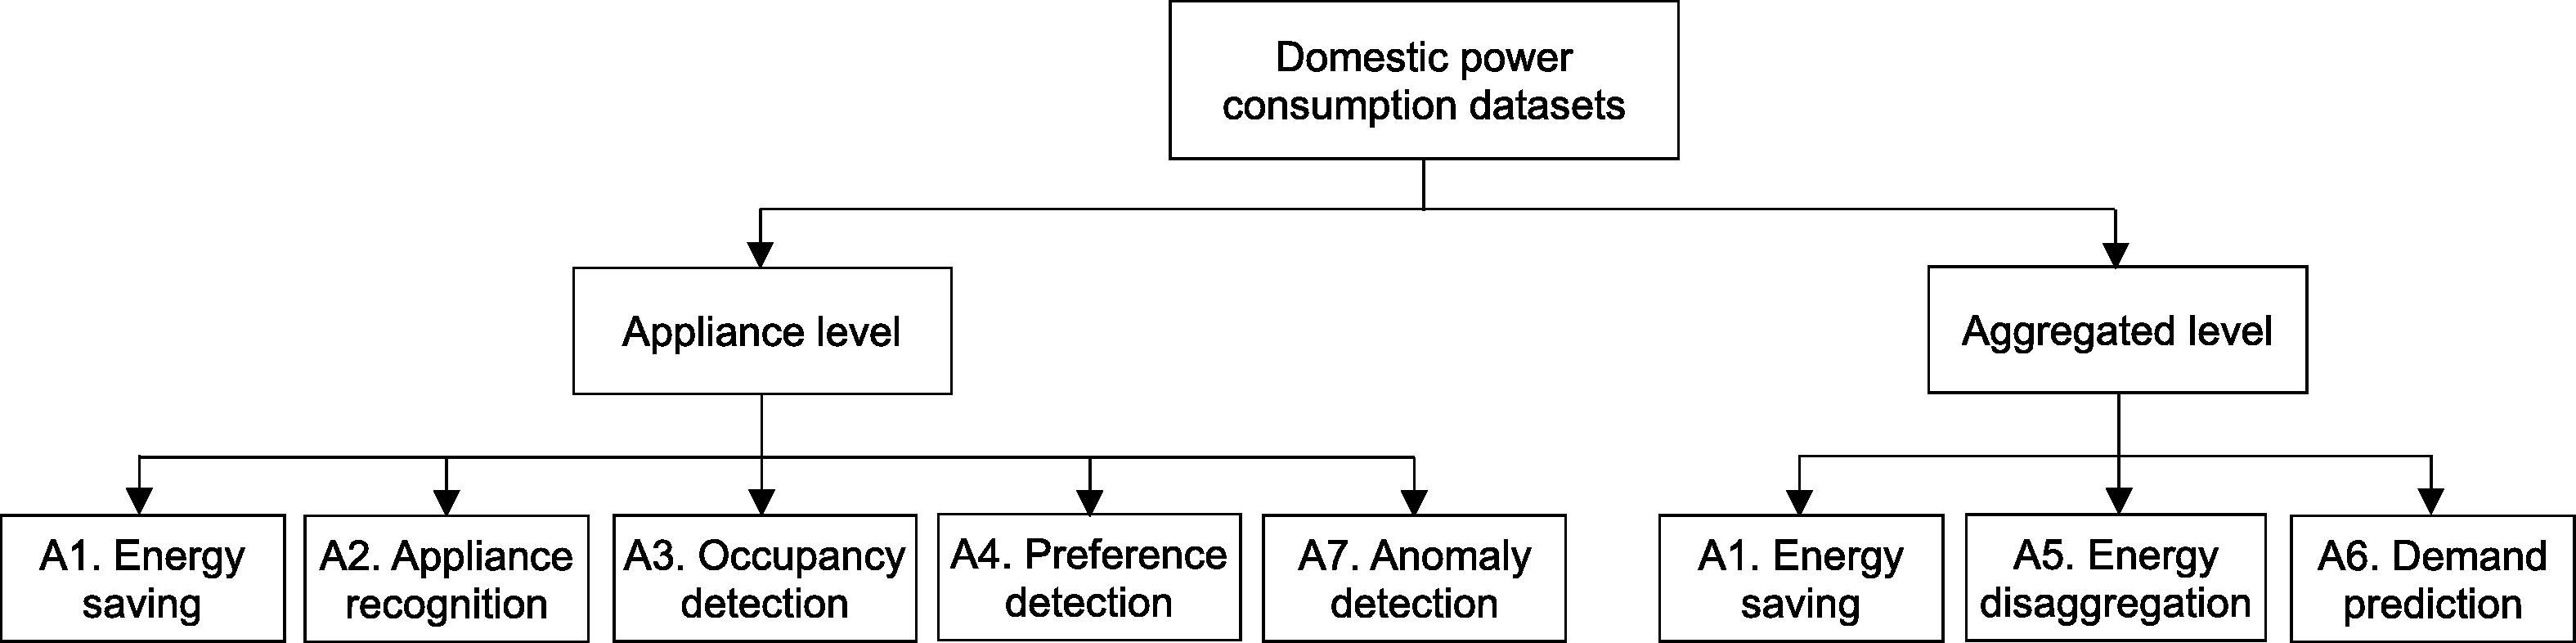
\includegraphics[width=.9\textwidth]{images/taxonomy_power_consumption.jpg}
    \caption[Applications of power consumption datasets]{Applications of power consumption datasets. From~\cite{himeur_building_2020}, page 5. CC-BY license.}
    \label{fig:applications_power_consumption_datasets}
\end{figure}

In~\parencite{himeur_building_2020}, various applications for power consumption datasets are proposed, of which a comprehensive overview illustrated in Figure~\ref{fig:applications_power_consumption_datasets}. It is worth noting that these applications are not mutually exclusive, and as such a single dataset may be appropriate for a number of uses. Application A7 (Anomaly Detection) is out of scope for this thesis, and no dataset for this application will be analyzed.

\newpage

\begin{enumerate}[label={\textit{A\arabic*.}}, leftmargin=3.5em]
    \item \textit{Energy Saving}. Investigating energy-saving measures in buildings can help reduce bills and lower carbon emissions, e.g. by deriving specific recommendations using \acrfull{ml} techniques in order to promote energy efficiency behaviors. Energy saving applications require the dataset to include data from various sources, including energy sub-meters, ambient condition sensors and climate sources.

    \item \textit{Appliance Recognition}. Identifying devices' power usage patterns can help in discriminating their operating conditions. This information can be used, for example, to recognize unattended appliances. 
    
    \item \textit{Occupancy Detection}. By analyzing power consumption profiles and environmental factors like temperature and humidity, it is possible to detect individuals' presence in specific building areas. The assessment of occupancy detection requires datasets with either aggregated or disaggregated power draw, along with a description of consumption scenarios. In particular, the presence of user-driven devices is needed to assume presence in the environment~\parencite{monacchi_greend_2014}.
    
    \item \textit{Preference Detection}, Analyzing energy usage profiles helps evaluate the preferences of occupants. \acrshort{ml} techniques interpret habits related to appliance usage of individuals, understanding their consumption priorities or creating contexts that satisfy their well-being. Datasets for preference detection require appliance-level power consumption.
    
    \item \textit{Energy Disaggregation}. Also named \acrfull{nilm} in the literature, it consists in separating overall power consumption into signals for individual electrical devices. \acrshort{ml} models can be used to learn the particular power consumption patterns of single devices, with the objective of discerning the contribution of single appliances to the total energy use when only the aggregate consumption data is given. Datasets for energy disaggregation need to include both aggregated and appliance-level consumption fingerprints, to compare the results obtained from disaggregation models with individual patterns of devices.
    
    \item \textit{Demand Prediction}. \acrshort{ml} algorithms can be used to forecast power demand, aiding public authorities, project managers, and homeowners in energy-efficient planning. Directives and mechanisms can be established in advance with a view of reducing load consumption of equipments and appliances inside infrastructures. Energy demand prediction benefits from power consumption data gathered over an extended collection period.

    \item \textit{Anomaly Detection}. Early detection methods can identify failures in devices and anticipate abnormal energy usage values. For anomaly detection, labeled datasets annotating normal and anomaly consumption footprints are needed.
\end{enumerate}

The frequency used for gathering the data can be significant for certain applications: in load disaggregation, a higher frequency allows for extraction of more representative features capturing the transient behavior~\parencite{carrie_armel_is_2013}. Geographical location is also significant, as in the USA nominal voltage in circuits is usually $120V$, while European countries commonly work under $230V$~\parencite{international_electrotechnical_commission_world_2024}.

The geographic location of the buildings where data is collected can be significant. Firstly, countries vary in their nominal voltages, with most European and some Asian countries setting single-phase nominal voltages in buildings to $230V$, while in the US and Canada, the value is $120V$~\parencite{lee_comparison_2017}. A lower nominal voltage implies that the maximum power draw of single appliances is limited. Additionally, factors like the level of development, climate, efficiency standards for appliance, or the stringency of building codes impact consumption patterns \parencite{berardi_cross-country_2017}.

\section{Overview of Power Consumption Datasets}

In this section a description of the characteristics power consumption datasets is provided, answering RQ3. An overview of the datasets is reported in Table~\ref{tab:datasets_overview}, while Table~\ref{tab:datasets_applications} compares the datasets in terms of resolution (both aggregate-level and appliance-level), features provided, and possible applications.

\subsection{REDD}

Released in 2011, the \acrlong{redd}\footnote{\url{https://tokhub.github.io/dbecd/links/redd.html}} is the first and most widely used public dataset in the history of energy disaggregation field~\parencite{iqbal_critical_2020}. It includes aggregated and appliance-specific electricity consumption data from six houses in Massachusetts, USA, collected over several months~\parencite{kolter_redd_2011}. Each monitored house provides two types of electricity data: the whole home signal, recorded with high-frequency monitors (15kHz) on both power phases and a voltage monitor on one phase, and 24 individual circuits labeled with appliance categories, recorded at a low frequency (0.5 Hz). Additionally, data of up to 20 plug-level monitors in the home recorded at 1 Hz is available, with a focus on logging electronics devices where multiple devices are grouped to a single circuit. Energy consumption data for the entire home and specific devices is available for one month. Finally \acrshort{redd} includes labels for the data where possible, which enables the use of supervised \acrshort{ml} approaches.

\subsection{HES}

Resulting from a UK government survey on 251 houses conducted between 2010 and 2011, the \acrlong{hes}\footnote{\url{https://www.gov.uk/government/publications/household-electricity-survey--2}} was released in 2012~\parencite{zimmermann_household_2012}. While 26 houses were monitored for a year, the rest were monitored for periods of one month at intervals throughout the year. \acrshort{hes}'s limitation is its 2-minute sampling frequency, which makes it inadequate for energy disaggregation as it will be difficult to differentiate between individual devices and occurrences \parencite{himeur_building_2020}. However, the dataset provides valuable property information for monitored homes, including building nature, size, room number, and occupants.

\subsection{Tracebase}

The Tracebase\footnote{\url{https://github.com/areinhardt/tracebase}} dataset for appliance identification comprises power consumption traces of individual appliances from 15 houses in Germany and Australia~\parencite{reinhardt_accuracy_2012}. Collected at a one-sample-per-second resolution, the dataset includes data from 43 distinct appliances, with various recordings spanning multiple days and households. The dataset was released in 2012, but the period during which the data was gathered is not known. While the dataset is valuable for energy efficiency applications, it lacks information on device properties, making it unsuitable for appliance recognition, preference detection, or energy disaggregation \parencite{himeur_building_2020}.

\subsection{Smart*}

The UMASS Smart* Home Dataset\footnote{\url{https://traces.cs.umass.edu/index.php/smart/smart}}, released in 2017, features non-continuous data from seven houses in Massachusetts, USA, over three years~\parencite{barker_smart_2012}. The dataset covers various sources, including electricity usage at mains panels, circuits, and plugs. Additionally, it includes data from weather, motion, door, wall switch, and thermostat sensors, along with electricity generation data from solar panels and wind turbines (every 5 seconds). The data was gathered in high-resolution: for electrical loads, real power each second for entire homes and each circuit is available, along with average real power from almost every individual plug load every few seconds. The dataset also captures on/off/dim events from wall switches and provides voltage and frequency measurements on both phases of the home’s split-leg input power.

\subsection{IHEPCDS}

The \acrlong{ihepcds}\footnote{\url{https://archive.ics.uci.edu/dataset/235/individual+household+electric+power+consumption}}~\parencite{georges_hebrail_individual_2006}, released in 2013, contains electricity measurements from a single home near Paris, France. Collected at a one-minute sampling rate, the data spans 47 months, from December 2006 to November 2010. The dataset presents various electrical quantities and sub-metering values, including current, voltage, active and reactive power, with different resolution features.

\subsection{GREEND}

The GREEND\footnote{\url{https://www.andreatonello.com/greend-energy-metering-data-set/}}~\parencite{monacchi_greend_2014} is a 1 Hz dataset resulting from a measurement campaign in the Carinthia region of Austria and the Friuli-Venezia Giulia region of Italy. The year-long campaign, started in December 2013, monitored nine houses, aiming to observe and model seasonal consumption behavior of inhabitants. The householders were selected in order to promote diversity of scenarios, for instance involving different types of dwellings and consumers. The dataset includes UTC Unix timestamps for eeasurements, allowing matching with contextual data such as weather.

\subsection{UK-DALE}

The UK-DALE dataset~\parencite{kelly_uk-dale_2015}\footnote{\url{https://jack-kelly.com/data/}} captures appliance-level electricity data from five UK houses. The sample rate is 16 kHz for whole-house consumption and 1/6 Hz for individual appliances. Various versions have been released, with the latest in 2017, covering 4.3 years. The houses were provided by MSc or PhD students from Imperial College, London, who chose the appliances to monitor, prioritizing the most energy-consuming ones as recommended by the authors.


\subsection{AMPds2}

The \acrlong{ampds2}\footnote{\url{https://dataverse.harvard.edu/dataset.xhtml?persistentId=doi:10.7910/DVN/FIE0S4}}~\parencite{makonin_electricity_2016} captures electricity, water, and natural gas consumption in a single house near Vancouver, Canada, over two years. The dataset provides 11 measurement characteristics for electricity and includes environmental and utility billing data for cost analysis. \acrshort{ampds2} data is pre-cleaned, with algorithmically filled missing data to maintain a continuous frequency of readings (once per minute). Eleven measurement characteristics of electricity for each meter were presented including active, reactive, and apparent power with other essential parameters.

\subsection{EMBED}

The \acrlong{embed}\footnote{\url{http://embed-dataset.org}}~\parencite{jazizadeh_embed_2018} dataset includes aggregate power measurements and plug load data of different appliances for three residential units in Los Angeles, USA. Collected over periods of two to four weeks, the dataset comprises raw current and voltage waveforms along with processed power metrics. \acrshort{embed} is suitable for comparing event-based and non-event-based methodologies, providing fully labeled disaggregation data where by separate labels are identified for different transition states for each appliance.

\subsection{PLAID}

The \acrlong{plaid}\footnote{\url{https://doi.org/10.6084/m9.figshare.10084619.v2}}~\parencite{medico_voltage_2020} contains records of electrical voltage and current from domestic appliances collected at a high sampling frequency of 30 kHz. This is the highest resolution frequency used in existing building power consumption datasets when collecting load profiles \parencite{himeur_building_2020}. All appliances are monitored individually: they are sub-metered and the data traces captured over a few seconds include the activation of the appliances. \acrshort{plaid} includes 1876 records from 17 appliance types comprising 330 different makes and models, collected at 65 locations in Pittsburgh, Pennsylvania, USA. Additionally, \acrshort{plaid} covers combined operation records (i.e., measurements obtained when multiple appliances were active simultaneously) and, for some appliances, multiple operating modes were monitored. The dataset does not include traces of active and reactive power.

\subsection{SynD}

SynD\footnote{\url{https://doi.org/10.6084/m9.figshare.c.4716179}} \parencite{klemenjak_synthetic_2020} is a synthetic dataset offering 180 days of  power data for 21 household appliances on both aggregate and per-appliance levels. The dataset, at a sampling frequency of 5 Hz, results from a simulation process based on power traces of real household appliances gathered through a measurement campaign in two households in the Carinthia region of Austria. A dataset generator was used with custom appliance models to simulate one household for given input parameters such as sampling rate and duration. The simulated household can be associated with a relaxed lifestyle of a single person or a young couple. SynD is validated against real appliance consumption for a period of forty days. However, it only considers active power, excluding apparent power, current, or voltage values.

\newpage

\subsection{DEDDIAG}

The \acrlong{deddiag}\footnote{\url{https://doi.org/10.6084/m9.figshare.13615073}}~\parencite{wenninger_deddiag_2021} includes recordings of domestic electricity demand of individual appliances from 15 homes in Germany over a period of up to 3.5 years. In particular, it covers 50 appliances at a 1 Hz frequency over periods of 21 to 1351 days. The dataset is designed for automated domestic load-shift applications. Hence, the dataset contains appliances that have the potential for automated load-shifting such as fridges, freezers, dishwashers, dryers and washing machines. One home also includes three-phase mains readings that can be used for disaggregation tasks. Additionally, \acrshort{deddiag} provides ground truth event annotations for 14 appliances, that provide precise start and stop timestamps. There are multiple labels per appliance where possible in order to annotate different modes. It also includes demographic data for each household's residents such as age, absence duration and regularity of absence.

\begin{table}
    \centering
    \resizebox{\textwidth}{!}{%
    \begin{tabular}{lllp{.1\textwidth}lp{.1\textwidth}lp{.14\textwidth}p{.65\textwidth}}
    \hline
        \textbf{\#} & \textbf{Dataset} & \textbf{Year} & \textbf{Location} & \textbf{Type} & \textbf{\# Houses} & \textbf{Period} & \textbf{\# Appliances} & \textbf{Appliances} \\ \hline
        1 & REDD & 2011 & USA & Real-world & 6 & 119 days & 19 & Furnace, outlets, washing machine, fridge, dish washer, lights, duct heater, dryer, microwave, AC, egauge, panel-GFI, tub, kitchen-counter, wine-cellar, garage-door, barn, well, solar \\ 
        2 & HES & 2011 & UK & Real-world & 251 & 1 year & 13 & Fridge, washing machine, washing dryer, dish washer, oven, cooker, hob, microwave oven, kettle, lighting, audiovisual site, television, space heating \\ 
        3 & Tracebase & 2012 & Australia & Real-world & 15 & - & 39 & DVD player, hifi-amplifier, subwoofer, vacuum cleaner, desk lamp, MacBook, monitor, alarm clock, amplifier, coffeemaker, breadcutter, cdplayer, charger, stove, TV, dishwasher, ethernet Switch, freezer, iron, dryer, oven, PC, laptop, toaster, USB hard drive, USB Hub, video projector, washing machine, water boiler, water fountain, water kettle, lights, play station, printer, projector, refrigerator, remote desktop, router, solar thermal system \\
        4 & Smart* & 2012 & USA & Real-world & 7 & 3 years & 19 & Furnace, outlets, washing machine, fridge, dish washer, lights, duct heater, dryer, microwave, AC, egauge, panel-GFI, tub, kitchen-counter, wine-cellar, garage-door, barn, well, solar \\
        5 & IHEPCDS & 2013 & France & Real-world & 1 & 47 months & 9 & Refrigerator, light, electric water heater, AC, dishwasher, oven, microwave, washing machine, tumble-drier \\
        6 & GREEND & 2014 & Austria, Italy & Real-world & 9 & 1 year & 27 & Coffee machine, washing machine, radio, water kettle, fridge, dishwasher, lamp, TV, vacuum cleaner, microwave, amplifier, lights, NAS, notebook, bread machine, outlets, hair dryer, computer, oven, scanner, printer, hood, toaster, stove, iron, decoder, ADSL modem \\
        7 & UK-DALE & 2015 & UK & Real-world & 5 & 4.3 years & 22 & Fridge freezer, home theatre PC, dish washer, washer dryer, kettle, AC, lamp, boiler,  breadmaker, soldering iron, computer monitor, toaster, television, vacuum cleaner, printer, ethernet switch, immersion heater, laptop computer, microwave, rice cooker, hair dryier, game console \\
        8 & AMPds2 & 2016 & Canada & Real-world & 1 & 2 years & 11 & Plugs \& lights, clothes dryer, clothes washer, dishwasher, fridge, furnace, garage, heat pump, instant hot Water unit, TV, oven \\
        9 & EMBED & 2018 & USA & Real-world & 3 & 2-4 weeks & 21 & Refrigerator, washing machine, central air conditioning (ac), window ac, toaster, kettle, tv, iron, hair dryer, hair iron, lcd monitor, laptop, light, grill, coffee maker, xbox, bathroom fan, water heater, surface tablet, microwave, electric range \\
        10 & PLAID & 2018 & USA & Real-world & 65 & 3 months & 16 & AC, blender, coffeemaker, Compact Fluorescent Lamp (CFL), fan, fridge, hair dryer, hair iron, heater, bulb, laptop, microwave, soldering iron, vacuum, washing machine, water kettle \\
        11 & SynD & 2020 & Austria & Synthetic & 2 & 180 days & 21 & Fridge, Dishwasher, Electric heater, Washing machine, Toaster, Fan, Microwave, Iron, Hot air gun, Router, Coffee machine, TV, Printer, Laptop computer, Lamp, Gaming PC, Pocket Radio, Monitor, Electric oven, Hair dryer, Water kettle \\
        12 & DEDDIAG & 2021 & Germany & Real-world & 15 & 3.5 years & 8 & Coffee machine, dish washer, dryer, freezer, office desk, refrigerator, tv, washing machine \\ \hline
    \end{tabular}}
    \caption{Overview of power consumption datasets.}
    \label{tab:datasets_overview}
\end{table}

\begin{table}
    \centering
    \resizebox{\textwidth}{!}{%
    \begin{tabular}{llllll}
        \hline
        \multirow{2}{*}{\#} & \multirow{2}{*}{Dataset} & \multicolumn{2}{l}{Resolution} & \multirow{2}{*}{Features} & \multirow{2}{*}{Applications} \\ \cline{3-4} &  & Aggregate & Appliance &  & \\ \hline
        1 & REDD & 15 kHz & 0.5 Hz, 1 Hz & I, V, P & A1, A2, A4, A5 \\
        2 & HES & 2 min or 10 min & 2 min or 10 min & I, V, P, T & A1, A6 \\
        3 & Tracebase & - & 1-8s & P, Np & A1, A6 \\
        4 & Smart* & 1 Hz & 1 Hz & I, V, P, f, S & A1, A2, A3, A4, A5, A6 \\
        5 & IHEPCDS & 1 min & 1 min & I, V, P, Q & A1, A6 \\
        6 & GREEND & 1 Hz & 1 Hz & P & A1, A2, A3, A4, A5, A6 \\
        7 & UK-DALE & 16 kHz & 1s, 6s & I, V, P, Q, S & A1, A2, A3, A4, A5, A6 \\
        8 & AMPds2 & 1 min & 1 min & I, V, P, S, f, pf & A1, A2, A4, A5 \\
        9 & EMBED & 12 kHz & 1 Hz & I, V, P, Q & A1, A2, A4, A5 \\
        10 & PLAID & - & 30 kHz & I, V & A1, A2, A4 \\
        11 & SynD & 5 Hz & 5 Hz & P & A1, A2, A4, A5 \\
        12 & DEDDIAG & 1 Hz & 1 Hz & P & A1, A2, A4, A5, A6 \\ \hline
    \end{tabular}}
    \caption[Comparison of power consumption datasets in terms of features, resolution, and applications]{Comparison of power consumption datasets in terms of features, resolution, and applications. The features reported are current (I), voltage (V), active power (P), reactive power (Q), apparent power (S), normalized power (Np), frequency (f), power factor (pf), and Temperature (T).}
    \label{tab:datasets_applications}
\end{table}